\documentclass[10pt]{article}
\usepackage{fullpage}
\usepackage{url}
\usepackage{color}
\usepackage{listings}

\definecolor{dkgreen}{rgb}{0,0.6,0}
\definecolor{dkred}{rgb}{0.6,0,0}
\definecolor{dkblue}{rgb}{0,0,0.7}

\usepackage{tikz}
\usetikzlibrary{automata, positioning, arrows}
\tikzset{%
  node distance=2.5cm,  
  initial text={},      
  every state/.style={  
    semithick},
  double distance=2pt,  % Accept state appearance
  every edge/.style={   
    draw,
    ->,
    >=stealth',
    auto,
    semithick} %
}

\lstdefinestyle{jvm}{
  % aboveskip=3mm,
  % belowskip=3mm,
  xleftmargin=2em,
  % xrightmargin=2em,
  showstringspaces=false,
  columns=flexible,
  basicstyle={\ttfamily},
  numbers=left,
  moredelim=[s][\color{black}]{Ljava}{;},
  morecomment=[l][\color{dkgreen}]{;},
  morecomment=[l][\color{magenta}]{;;},
  keywords={class,public,static,super,method,code,end},
  keywordstyle=\color{dkblue},
  breaklines=true,
  breakatwhitespace=true,
  tabsize=8
}

\renewcommand{\thepage}{~}

\title{COM S 440/540 Homework 2}
\date{}
\author{Lexical Analysis 2}

\begin{document}

\maketitle

\noindent
Reminder: present your own work and properly cite any sources used.
Solutions should be written satisfying the \emph{other student viewpoint},
and must be prepared using \LaTeX.
\renewcommand{\thepage}{~}
 
%============================================================
\section*{Question~1~\hfill 15--20 points}
%============================================================

\begin{center}
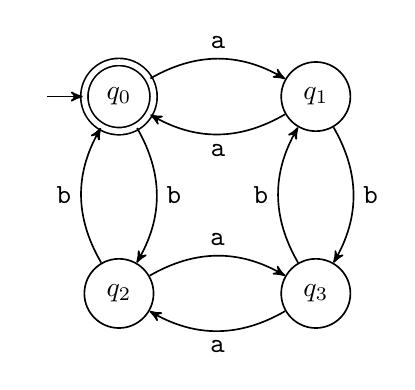
\begin{tikzpicture}
  \node[state, accepting, initial] (q0) {$q_0$};
  \node[state, right of=q0] (q1) {$q_1$};
  \node[state, below of=q0] (q2) {$q_2$};
  \node[state, right of=q2] (q3) {$q_3$};

  \draw 
        (q0) edge [bend left, above] node{{\tt a}} (q1)
        (q1) edge [bend left, below] node{{\tt a}} (q0)

        (q0) edge [bend left, right] node{{\tt b}} (q2)
        (q2) edge [bend left,  left] node{{\tt b}} (q0)

        (q2) edge [bend left, above] node{{\tt a}} (q3)
        (q3) edge [bend left, below] node{{\tt a}} (q2)

        (q1) edge [bend left, right] node{{\tt b}} (q3)
        (q3) edge [bend left,  left] node{{\tt b}} (q1)
  ;

\end{tikzpicture}
\end{center}
Consider the NFA shown above.
\begin{enumerate}
\item
For each word shown below, is it accepted by the NFA or not?
Explain why.
\begin{itemize}
  \item `` '' (empty string)
  \item ``{\tt ba}''
  \item ``{\tt ababa}''
  \item ``{\tt bbbaba}''
  \item ``{\tt baabba}''
\end{itemize}

\item
{\bf (Extra credit for 440) }
Describe, in English, which words are accepted.
\end{enumerate}


%============================================================
\section*{Question~2~\hfill 20 points}
%============================================================

Draw, or formally define, 
an NFA that accepts well-formed C comments
(i.e., comments that begin with \verb|/*|
and end with \verb|*/|).
Use the set of ASCII characters as the alphabet $\Sigma$.
The following are examples of words that should be accepted.
\begin{verbatim}
  /**/
  /******/
  /* This is a comment */
  /* This is a\n\tmulti-line comment */
\end{verbatim}

\end{document}
